\documentclass[fleqn]{article}
\oddsidemargin 0.0in
\textwidth 6.0in
\thispagestyle{empty}
\usepackage{import}
\usepackage{amsmath}
\usepackage{graphicx}
\usepackage{flexisym}
\usepackage{amssymb}
\usepackage{bigints} 
\usepackage[english]{babel}
\usepackage[utf8x]{inputenc}
\usepackage{float}
\usepackage[colorinlistoftodos]{todonotes}

\definecolor{hwColor}{HTML}{AD53BA}

\begin{document}

  \begin{titlepage}

    \newcommand{\HRule}{\rule{\linewidth}{0.5mm}}

    \center


    \textsc{\LARGE Arizona State University}\\[1.5cm]

    \textsc{\LARGE Linear Algebra }\\[1.5cm]


    \begin{figure}
      
\includegraphics[width=\linewidth]{asu.png}
    \end{figure}


    \HRule \\[0.4cm]
    { \huge \bfseries Quiz Four}\\[0.4cm] 
    \HRule \\[1.5cm]

    \textbf{Behnam Amiri}

    \bigbreak

    \textbf{Prof: Sergei Suslov}

    \bigbreak


    \textbf{{\large \today}\\[2cm]}

    \vfill

  \end{titlepage}

  \begin{enumerate}
    \item (10 points) Find the angle between the vectors $u=(-1, 2, -3, 4)$ and $v=(1, -3, 2, -4)$ and 
    verify the Cauchy-Schwarz inequality, $|\left\langle u, v\right\rangle| \leq ||u|| ~ ||v||$, for 
    them using the standard inner product in $\mathbb{R}^4: ~ \left\langle u,v\right\rangle =u_1 v_1+u_2 v_2+u_3 v_3+u_4 v_4$.

      \textcolor{hwColor}{
        $
          \\
          \\
          \begin{cases}
              \left\langle \overrightarrow{u}.\overrightarrow{v}\right\rangle=(-1)(1)+(2)(-3)+(-3)(2)+(4)(-4)=-29
              \\
              \\
              ||\overrightarrow{u}||^2=\left\langle \overrightarrow{u}.\overrightarrow{u}\right\rangle=(-1)^2+(2)^2+(-3)^2+(4)^2=30 \longrightarrow ||\overrightarrow{u}||=\sqrt{30}
              \\
              \\
              ||\overrightarrow{v}||^2=\left\langle \overrightarrow{v}.\overrightarrow{v}\right\rangle=(1)^2+(-3)^2+(2)^2+(-4)^2=30 \longrightarrow ||\overrightarrow{v}||=\sqrt{30}
          \end{cases}
          \\
          \\
          \\
          cos(\theta)=\dfrac{\left\langle \overrightarrow{u}.\overrightarrow{v}\right\rangle}{||\overrightarrow{u}||||\overrightarrow{v}||}
          =-\dfrac{29}{\sqrt{30} \sqrt{30}}
          =-\dfrac{29}{30}
          \\
          \\
          \therefore ~~~~ \theta=arccos(-\dfrac{29}{30}) \approx 165^{\circ}
          \\
          \\
          \\
          |\left\langle u, v\right\rangle| \leq ||u|| ~ ||v|| \Longrightarrow 29 \leq \sqrt{30} \sqrt{30} \Longrightarrow 29 \leq 30
        $
        \\
        \\
        As it is shown the Cauchy-Schwarz inequality holds. $\blacksquare$
      }

    \item (10 points) Verify that the set of three vectors $v_1=(0, 1, 0), v_2=(-\dfrac{5}{13}, 0, \dfrac{12}{13}),$ and \\
    $v_3=(\dfrac{12}{13}, 0, \dfrac{5}{13})$ forms an orthonormal basis for $\mathbb{R}^3$ with the standard Euclidean inner
    product. Express the vector $u=(1, 2, 3)$ as a linear combination of the vectors in the given set: 
    $u=c_1 v_1+c_2 v_2+c_3 v_3$ and find the coordinates $c_1, c_2$ and $c_3$.

      \textcolor{hwColor}{
        \\
        Based on the given vectors, let's create a set of column space: 
        $$
          S=\{ \left(0, 1, 0\right), \left(-\dfrac{5}{13}, 0, \dfrac{12}{13}\right), \left(\dfrac{12}{13}, 0, \dfrac{5}{13}\right) \} 
        $$
        Now let's find the inner product of these vectors: 
        \\
        \\
        $
          \begin{cases}
            \left\langle v_1, v_2\right\rangle=(0)(-\dfrac{5}{13})+(1)(0)+(0)(\dfrac{12}{13})=0
            \\
            \\
            \left\langle v_1, v_3\right\rangle=(0)(\dfrac{12}{13})+(1)(0)+(0)(\dfrac{5}{13})=0
            \\
            \\
            \left\langle v_2, v_3\right\rangle=(-\dfrac{5}{13})(\dfrac{12}{13})+(0)(0)+(\dfrac{12}{13})(\dfrac{5}{13})=0
          \end{cases}
        $
        \\
        \\
        These results show that the given vectors are linearly independent, therefore they form a basis for $\mathbb{R}^3$.
        Also, it is obvious that the given vectors are orthogonal to each other, therefore the set $S$ is an orthogonal
        set in $\mathbb{R}^3$. 
        \\
        \\
        \\
        $
          \begin{cases}
            ||v_1||=\sqrt{(0)^2+(1)^2+(0)^2}=1
            \\
            \\
            ||v_2||=\sqrt{(-\dfrac{5}{13})^2+(0)^2+(\dfrac{12}{13})^2}=1
            \\
            \\
            ||v_3||=\sqrt{(\dfrac{12}{13})^2+(0)^2+(\dfrac{5}{13})^2}=1
          \end{cases}
        $
        \\
        \\
        Therefore, the set $S$ is orthonormal.
        \\
        \\
        Time to find the coordinates $c_1, c_2,$ and $c_3$.
        \\
        \\
        $
          u=c_1 v_1+c_2 v_2+c_3 v_3 \Longrightarrow (1, 2, 3)=c_1 (0, 1, 0)+c_2 (-\dfrac{5}{13}, 0, \dfrac{12}{13})+c_3 (\dfrac{12}{13}, 0, \dfrac{5}{13})
          \\
          \\
          \\
          \Longrightarrow (1, 2, 3)=(0, c_1, 0)+(-\dfrac{5}{13}c_2, 0, \dfrac{12}{13}c_2)+(\dfrac{12}{13}c_3, 0, \dfrac{5}{13}c_3)
          \\
          \\
          \\
          \begin{cases}
            -\dfrac{5}{13}c_2+\dfrac{12}{13}c_3=1
            \\
            \\
            c_1=2
            \\
            \\
            \dfrac{12}{13}c_2+\dfrac{5}{13}c_3=3 
          \end{cases} \Longrightarrow
          \begin{cases}
            -\dfrac{5}{13}c_2+\dfrac{12}{13}c_3=1
            \\
            \\
            \dfrac{12}{13}c_2+\dfrac{5}{13}c_3=3 
          \end{cases} \Longrightarrow 
          \left(\begin{array}{cc|c}  
            -\dfrac{5}{13} & \dfrac{12}{13} & 1
            \\
            \\
            \dfrac{12}{13} & \dfrac{5}{13} & 3
          \end{array}\right)
          \\
          \\
          \rule{15cm}{3pt}
          \\
          \\
          -\dfrac{13}{5}R_1 \rightarrow R_1
          \\
          \\
          \left(\begin{array}{cc|c}  
            1 & -\dfrac{12}{5} & -\dfrac{13}{5}
            \\
            \\
            \dfrac{12}{13} & \dfrac{5}{13} & 3
          \end{array}\right)
          \\
          \\
          \rule{15cm}{3pt}
          \\
          \\
          -\dfrac{12}{13}R_1+R_2 \rightarrow R_2
          \\
          \\
          \left(\begin{array}{cc|c}  
            1 & -\dfrac{12}{5} & -\dfrac{13}{5}
            \\
            \\
            0 & \dfrac{13}{5} & \dfrac{27}{5}
          \end{array}\right)
          \\
          \\
          \rule{15cm}{3pt}
          \\
          \\
          \dfrac{5}{13}R_2 \rightarrow R_2
          \\
          \\
          \left(\begin{array}{cc|c}  
            1 & -\dfrac{12}{5} & -\dfrac{13}{5}
            \\
            \\
            0 & 1 & \dfrac{27}{13}
          \end{array}\right)
          \\
          \\
          \rule{15cm}{3pt}
          \\
          \\
          \dfrac{12}{5}R_2+R_1 \rightarrow R_1
          \\
          \\
          \left(\begin{array}{cc|c}  
            1 & 0 & \dfrac{31}{13}
            \\
            \\
            0 & 1 & \dfrac{27}{13}
          \end{array}\right)
          \\
          \\
          \\
          \therefore ~~~~~ \begin{cases}
            c_1=2
            \\
            \\
            c_2=\dfrac{31}{13}
            \\
            \\
            c_3=\dfrac{27}{13}
          \end{cases} ~~~~~ \checkmark
        $
      }

    \item (10 points) Prove the Cauchy-Schwarz inequality, $|\left\langle u, v\right\rangle| \leq ||u|| ~ ||v||$,
    for two arbitrary vectors in an abstract inner product space $V$. Write this inequality explicitly in $\mathbb{R}^4$
    with the standard inner product: $\left\langle u,v\right\rangle =u_1 v_1+u_2 v_2+u_3 v_3+u_4 v_4$.

      \textcolor{hwColor}{
        There are two possibilities $\begin{cases}
          u=0
          \\
          u \neq 0
        \end{cases}$. Let's consider the two cases.
        \\
        \\
        \\
        \textbf{Case 1: $u=0$}
        \\
        \\
        $
          <u, v>=<0, v>=0, ~~~~ ||u||=\sqrt{<u, u>}=\sqrt{<0,0>}=0
          \\
          \\
        $
        Therefore, both sides of $|\left\langle u, v\right\rangle| \leq ||u|| ~ ||v||$ are equal to zero.
        which 
        \\
        \\
        \rule{15cm}{3pt}
        \\
        \\
        \textbf{Case 2: $u \neq 0$}
        \\
        \\
        Let's have $u \neq 0$ and $z=v-\dfrac{<v,u>}{||u||^2}u$.
        \\
        \\
        $
          <z.z>=<v-\dfrac{<v,u>}{||u||^2}u, v-\dfrac{<v,u>}{||u||^2}u>
          \\
          \\
          \\
          =<v,v>-\dfrac{<v, u><v,u>}{||u||^2}-\dfrac{<v,u><u,v>}{||u||^2}+<u,u>\dfrac{<v,u><v,u>}{||u||^4}
          \\
          \\
          \\
          =<v,v>-\dfrac{<v,u><v,u>}{||u||^2}-\dfrac{<u,v><u,v>}{||u||^2}+\dfrac{<v,u><v,u>}{||u||^2}
          \\
          \\
          \\
          =||v||^2-\dfrac{|<u,v>|^2}{||u||^2}
          \\
          \\
          \\
          =\dfrac{||u||^2 ~ ||v||^2-|<u,v>|^2}{||u||^2}
        $
        \\
        \\
        Based on the above result:
        \\
        \\
        $
          \therefore ~~~~~ \left\langle z,z\right\rangle  \geq 0
          \\
          \\
          \Longrightarrow \dfrac{||u||^2 ~ ||v||^2-|<u,v>|^2}{||u||^2} \geq 0
          \\
          \\
          \Longrightarrow ||u||^2 ~ ||v||^2-|<u,v>|^2 \geq 0
          \\
          \\
          \Longrightarrow |\left\langle u,v\right\rangle| \leq ||u|| ~ ||v|| ~~~~ \checkmark
        $
        \\
        \\
        In $\mathbb{R}^4$ with standard inner product we have:
        \\
        \\
        $
          \left\langle u,v\right\rangle=u_1 v_1+u_2 v_2+u_3 v_3+u_4 v_4
          \\
          \\
          |\left\langle u,v\right\rangle|=|u_1 v_1+u_2 v_2+u_3 v_3+u_4 v_4|
          \\
          \\
          \begin{cases}
            ||u||=\sqrt{\left\langle u,u\right\rangle}=\sqrt{u_1^2+u_2^2+u_3^2+u_4^2}
            \\
            \\
            ||v||=\sqrt{\left\langle u,u\right\rangle}=\sqrt{v_1^2+v_2^2+v_3^2+v_4^2}
          \end{cases}
        $
        \\
        \\
        \\
        Almost there. We need to rewrite the above inequality so we get:
        \\
        \\
        $
          |u_1 v_1+u_2 v_2+u_3 v_3+u_4 v_4| \leq \sqrt{u_1^2+u_2^2+u_3^2+u_4^2} \sqrt{v_1^2+v_2^2+v_3^2+v_4^2}
          \\
          \\
          \\
          \therefore ~~~~ |u_1 v_1+u_2 v_2+u_3 v_3+u_4 v_4| \leq \sqrt{\left(u_1^2+u_2^2+u_3^2+u_4^2\right) \left(v_1^2+v_2^2+v_3^2+v_4^2\right)} ~~~ \blacksquare 
        $
      }

    \pagebreak

    \item (10 points) Convert the basis $v_1=(1, -1, 0), v_2=(0, 1, -1),$ and $v_3=(-1, 1, -1)$ for $\mathbb{R}^3$ into
    an orthonormal basis, using the Gram-Schmidt process and the standard inner product in $\mathbb{R}^3$.

      \textcolor{hwColor}{
        The Gram-Schmidt process (or procedure) is a sequence of operations that allow to transform
        a set of linearly independent vectors into a set of orthonormal vectors that span the same space
        spanned by the original set.
        \\
        \\
        $
          \begin{cases}
            u_1=\dfrac{v_1}{||v_1||}
            \\
            \\
            u_2=\dfrac{v_2-(u_1.u_2)u_1}{||v_2-(u_1.u_2)u_1||}
            \\
            \\
            u_3=\dfrac{v_3-(u_2.v_3)u_2-(u_1.v_3)u_1}{||v_3-(u_2.v_3)u_2-(u_1.v_3)u_1||}
          \end{cases}
          \\
          \\
          \rule{15cm}{1pt}
          \\
          \\
          u_1: 
          \\
          \\
          u_1=\dfrac{(1, -1, 0)}{\sqrt{(1)^2+(-1)^2+(0)^2}}=\dfrac{(1, -1, 0)}{\sqrt{2}}=(\dfrac{1}{\sqrt{2}}, -\dfrac{1}{\sqrt{2}}, 0)
          \\
          \\
          \rule{15cm}{1pt}
          \\
          \\
          u_2:
          \\
          \\
          u_2=\dfrac{v_2-(u_1.v_2)u_1}{||v_2-(u_1.v_2)u_1||}=\dfrac{(0, 1, -1)-\left[(\dfrac{1}{\sqrt{2}}, -\dfrac{1}{\sqrt{2}}, 0).(0, 1, -1)\right](\dfrac{1}{\sqrt{2}}, -\dfrac{1}{\sqrt{2}}, 0)}{||(0, 1, -1)-\left[(\dfrac{1}{\sqrt{2}}, -\dfrac{1}{\sqrt{2}}, 0).(0, 1, -1)\right](\dfrac{1}{\sqrt{2}}, -\dfrac{1}{\sqrt{2}}, 0)||}
          \\
          \\
          \\
          u_2=\dfrac{(0, 1, -1)-(-\dfrac{1}{2}, \dfrac{1}{2}, 0)}{||(0, 1, -1)-(-\dfrac{1}{2}, \dfrac{1}{2}, 0)||}
          =\dfrac{(\dfrac{1}{2},\dfrac{1}{2},-1)}{||(\dfrac{1}{2},\dfrac{1}{2},-1)||}
          =\dfrac{(\dfrac{1}{2},\dfrac{1}{2},-1)}{\sqrt{(\dfrac{1}{2})^2+(\dfrac{1}{2})^2+(-1)^2}}
          \\
          \\
          \\
          u_2=\dfrac{(\dfrac{1}{2},\dfrac{1}{2},-1)}{\sqrt{\dfrac{3}{2}}}=\sqrt{\dfrac{2}{3}}(\dfrac{1}{2},\dfrac{1}{2},-1)=(\dfrac{1}{\sqrt{6}}, \dfrac{1}{\sqrt{6}},-\sqrt{\dfrac{2}{3}})
          \\
          \\
          \rule{15cm}{1pt}
          \\
          \\
          u_3:
          \\
          \\
          u_3=\dfrac{v_3-(u_2.v_3)u_2-(u_1.v_3)u_1}{||v_3-(u_2.v_3)u_2-(u_1.v_3)u_1||}
          \\
          \\
          =\dfrac{(-1, 1, -1)-\left[(\dfrac{1}{\sqrt{6}}, \dfrac{1}{\sqrt{6}},-\sqrt{\dfrac{2}{3}}).(-1, 1, -1)\right](\dfrac{1}{\sqrt{6}}, \dfrac{1}{\sqrt{6}},-\sqrt{\dfrac{2}{3}})-\left[(\dfrac{1}{\sqrt{2}}, -\dfrac{1}{\sqrt{2}}, 0).(-1, 1, -1)\right](\dfrac{1}{\sqrt{2}}, -\dfrac{1}{\sqrt{2}}, 0)}{||(-1, 1, -1)-\left[(\dfrac{1}{\sqrt{6}}, \dfrac{1}{\sqrt{6}},-\sqrt{\dfrac{2}{3}}).(-1, 1, -1)\right](\dfrac{1}{\sqrt{6}}, \dfrac{1}{\sqrt{6}},-\sqrt{\dfrac{2}{3}})-\left[(\dfrac{1}{\sqrt{2}}, -\dfrac{1}{\sqrt{2}}, 0).(-1, 1, -1)\right](\dfrac{1}{\sqrt{2}}, -\dfrac{1}{\sqrt{2}}, 0)||}
        $
        \\
        \\
        \\
        After doing some messy algebra we get $u_3=\left(-\dfrac{1}{\sqrt{3}}, -\dfrac{1}{\sqrt{3}}, -\dfrac{1}{\sqrt{3}}\right)$
        \\
        \\
        \\
        $
          \therefore ~~~~ \begin{cases}
            u_1=\left(\dfrac{1}{\sqrt{2}}, -\dfrac{1}{\sqrt{2}}, 0\right)
            \\
            \\
            u_2=\left(\dfrac{1}{\sqrt{6}}, \dfrac{1}{\sqrt{6}},-\sqrt{\dfrac{2}{3}}\right)
            \\
            \\
            u_3=\left(-\dfrac{1}{\sqrt{3}}, -\dfrac{1}{\sqrt{3}}, -\dfrac{1}{\sqrt{3}}\right)
          \end{cases} ~~~~ \checkmark
        $
      }

    \item (Extra credit, 5 points) The linear transformation, $L \left[p(x)\right]=\dfrac{d}{dx}p(x)+p(0)$, maps 
    a polynomial $p(x)$ of degree $\leq 2$  into a polynomial of degree $\leq 1$, namely, $L: P_2 \rightarrow P_1$.
    Find the matrix representation of $L$ with respect to the ordered bases $\{ x^2, x, 1\}$ and $\{ x, 1\}$.

      \textcolor{hwColor}{
        Let $f(x)=ax^2+bx+c$ and $g(x)=px^2+qx+d$ then:
        \\
        \\
        $
          L\left[f(x)\right]=\dfrac{d}{dx} f(x)+f(0)=2ax+b+c
          \\
          \\
          L\left[g(x)\right]=\dfrac{d}{dx}g(x)+g(0)=2px+q+d
          \\
          \\
          \\
          L\left[\alpha f(x)+\beta g(x)\right]
          =L\left[(\alpha a+\beta p)x^2+(\alpha b+\beta q)x+(\alpha c+\alpha d)\right]
          \\
          \\
          =\alpha (2ax+b+c)+\beta (2px+q+d)
          \\
          \\
          =\alpha L(f(x))+\beta L(g(x)) ~~~~ \checkmark
        $
        \\
        \\
        What we just found is a linear transformation from $P_2 \rightarrow P_1$.
        \\
        \\
        \\
        $
          \begin{cases}
            L(x^2)=\dfrac{d}{dx}x^2+0=2x
            \\
            \\
            L(x)=\dfrac{d}{dx}x+0=1
            \\
            \\
            L(1)=\dfrac{d}{dx}1+1  
          \end{cases} \Longrightarrow \begin{pmatrix}
            2 & 0 & 0
            \\
            0 & 1 & 1
          \end{pmatrix} ~~~~ \checkmark
        $
      }

    \item (10 points) Show that for any two vectors $u$ and $v$ in an inner product space $V$,
    $$||u+v||^2+||u-v||^2=2\left(||u||^2+||v||^2\right)$$
    Give a geometric interpretation of this result for the vector space $\mathbb{R}^2$.

      \textcolor{hwColor}{
        We can start off from the right side of the given statement.
        \\
        \\
        $
          ||u+v||^2=\left\langle u+v, u+v\right\rangle
          \\
          \\
          =\left\langle u, u+v\right\rangle+\left\langle v, u+v\right\rangle 
          \\
          \\
          =\left[\left\langle u, u\right\rangle+\left\langle u, v\right\rangle\right]+\left[\left\langle v, u\right\rangle+ \left\langle v, v\right\rangle \right]
          \\
          \\
          \\
          \therefore ~~~~ ||u+v||^2=||u||^2+\left\langle u, v\right\rangle+\left\langle v, u\right\rangle+||v||^2 ~~~~ \checkmark ~~~~ (A)
          \\
          \\
          \rule{15cm}{1pt}
          \\
          \\
          ||u-v||^2=\left\langle u-v, u-v\right\rangle
          \\
          \\
          =\left\langle u, u-v\right\rangle+\left\langle v, u-v\right\rangle 
          \\
          \\
          =\left[\left\langle u, u\right\rangle+\left\langle u, v\right\rangle\right]-\left[\left\langle v, u\right\rangle- \left\langle v, v\right\rangle \right]
          \\
          \\
          \\
          \therefore ~~~~ ||u-v||^2=||u||^2-\left\langle u, v\right\rangle-\left\langle v, u\right\rangle+||v||^2 ~~~~ \checkmark ~~~~ (B)
        $
        \\
        \\
        From (A) and (B) we have:
        \\
        \\
        $
          ||u+v||^2+||u-v||^2=\left[||u||^2+\left\langle u, v\right\rangle+\left\langle v, u\right\rangle+||v||^2\right]+\left[||u||^2-\left\langle u, v\right\rangle-\left\langle v, u\right\rangle+||v||^2\right]
          \\
          \\
          \\
          \therefore ~~~~ ||u+v||^2+||u-v||^2=2 \left[||u||^2+||v||^2\right] ~~~~ \checkmark
        $
        \\
        \\
        \\
        \textbf{Geometric interpretation:}
        \\
        \\
        Parallelogram law states that the sum of the squares of the length of the four sides of a parallelogram is 
        equal to the sum of the squares of the length of the two diagonals. In Euclidean geometry, it is necessary that 
        the parallelogram should have equal opposite sides.
        \\
        \\
        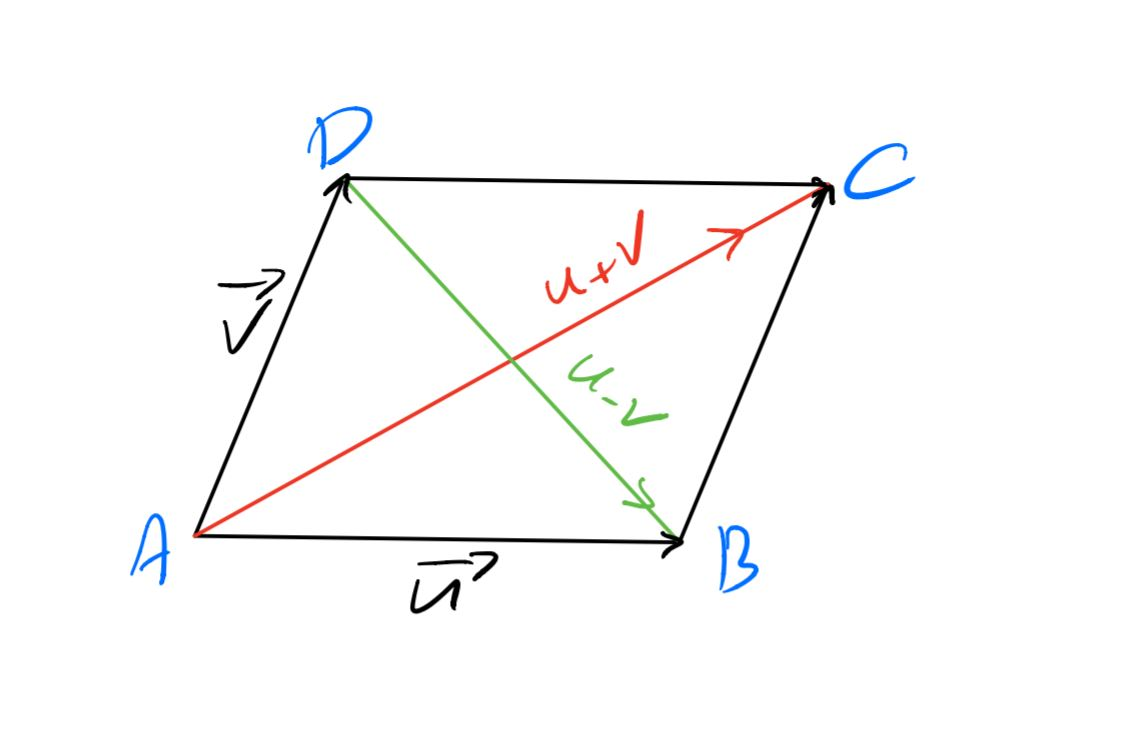
\includegraphics[height=6cm, width=10cm]{Yah.JPG}
        \\
        \\
        \\
        Let $u=\overrightarrow{AB}, v=\overrightarrow{BC}$ therefore $||u||=AB$ and $||v||=BC$.
        \\
        \\
        The vectors $u+v$ and $u-v$ represent the diagonals $\overrightarrow{AC}$ and $\overrightarrow{DB}$ of
        parallelogram $ABCD$. Note that $||u+v||=AC$ and $||u-v||=DB$.
        \\
        \\
        $
          ||u+v||^2+||u-v||^2=2\left(||u||^2+||v||^2\right)
          \\
          \\
          \Longrightarrow AC^2+DB^2=2\left(AB^2+BC^2\right)=AB^2+BC^2+CD^2+DA^2 ~~~~~ \checkmark
        $
      }

  \end{enumerate}

\end{document}
